% Drawing 83/01-1 -- folder 83, batch 01, archive page 5 (PDF page 6).
% Transcription: un carré encadré : $u$ — $uv$ en haut, $1$ — $v$ en bas, avec deux diagonales parallèles $1$–$u$ et $v$–$uv$.
% Kind: framed square with two parallel diagonals. Method 2 (schematic redraw from the facsimile). Status: ok.
% Notes: In a drawn frame: u (top left) - uv (top right), 1 (bottom left) - v (bottom right); short strokes for the sides u-uv and 1-v and the two parallel diagonals 1-u and v-uv. The vertical sides are not drawn.
% Coordinates: 1 unit = 1 mm = 1/100 of the crop width (bbox in page fractions: [0.32, 0.4, 0.56, 0.52]).
% Redrawn by Claude (claude-opus-5-5), issue #73, 2026-11-07; not checked by a human; not compiled (no TeX in the session).
% Rights: reproduces part of the work -- behind RENDER_TRANSCRIPTS, never published by itself.
\documentclass[tikz,border=3pt]{standalone}
\usepackage{amsmath,amssymb}
\usetikzlibrary{patterns,arrows.meta}
\tikzset{pencil/.style={black!45}, struck/.style={black!35}, mark/.style={circle,draw,inner sep=1.3pt}, pt/.style={circle,fill,inner sep=0.9pt}, opt/.style={circle,draw,fill=white,inner sep=1.1pt}}
\begin{document}
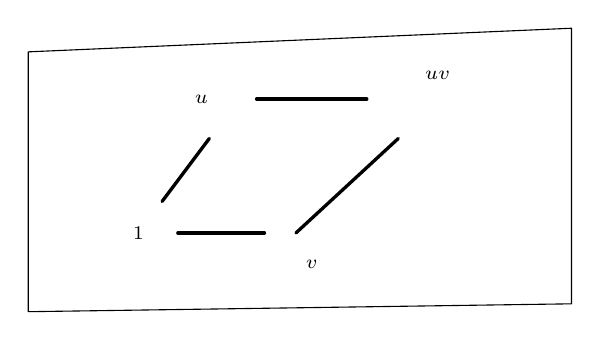
\begin{tikzpicture}[x=1mm,y=1mm,line cap=round,line join=round,font=\scriptsize]
\draw (13,-25) -- (82,-22) -- (82,-57) -- (13,-58) -- cycle;
\draw[very thick] (42,-31) -- (56,-31);
\draw[very thick] (32,-48) -- (43,-48);
\draw[very thick] (30,-44) -- (36,-36);
\draw[very thick] (47,-48) -- (60,-36);
\node[inner sep=1pt] at (35,-31) {\scriptsize $u$};
\node[inner sep=1pt] at (65,-28) {\scriptsize $uv$};
\node[inner sep=1pt] at (27,-48) {\scriptsize $1$};
\node[inner sep=1pt] at (49,-52) {\scriptsize $v$};
\end{tikzpicture}
\end{document}
